\documentclass[border=3pt]{standalone}
% Preâmbulo compartilhado pelos diagramas TikZ da aula 6 de IHC (Necessidades e Requisitos)
\usepackage[T1]{fontenc}
\usepackage[utf8]{inputenc}
\usepackage{lmodern}
\usepackage{amsmath}
\usepackage{xcolor}
\usepackage{tikz}
\usetikzlibrary{arrows.meta,angles,quotes,decorations.pathmorphing,calc,
                positioning,shapes.geometric,shapes.misc,backgrounds,fit,
                math}

% Paleta (mesma dos SVGs originais)
% Paleta da disciplina de IHC: acento roxo (#755099), da capa do livro.
% (o nome "dblue" é mantido para não alterar todos os diagramas)
\definecolor{dblue}{HTML}{755099}
\definecolor{dorange}{HTML}{B3541E}
\definecolor{dgreen}{HTML}{4A7C59}
\definecolor{dred}{HTML}{9C4B4B}
\definecolor{dcream}{HTML}{F4F1EA}
\definecolor{dshade}{HTML}{DDD7C9}

% Função gaussiana (não normalizada por padrão de escala visual)
\pgfmathdeclarefunction{gauss}{3}{%
  \pgfmathparse{1/(#3*sqrt(2*pi))*exp(-((#1-#2)^2)/(2*#3^2))}%
}

% Estilos comuns (prefixo d... para não colidir com chaves internas do pgf)
\tikzset{
  >={Stealth[length=2mm]},
  dguide/.style={gray!55, dashed, line width=0.4pt},
  daxis/.style={gray!60, line width=0.7pt, ->},
  dbody/.style={fill=black!3, draw=black!80, line width=1pt},
  dacc/.style={draw=dblue, line width=1pt},
  dlbl/.style={black!55, font=\small},
  dsub/.style={black!45, font=\footnotesize},
  dstate/.style={circle, draw=black!80, fill=dcream, line width=1pt,
                 minimum size=17mm, font=\large, inner sep=1pt},
  dobs/.style={circle, draw=black!80, fill=dshade, line width=1pt,
               minimum size=14mm, font=\large, inner sep=1pt},
  dbox/.style={rounded corners=2pt, draw=black!80, fill=dcream, line width=1pt,
               align=center, inner sep=6pt},
  dop/.style={circle, draw=black!80, fill=white, line width=1pt,
              minimum size=6mm, inner sep=0pt, font=\small},
  dtrans/.style={->, dblue, line width=1pt},
  dmeas/.style={->, dorange, line width=1pt},
  dcurve/.style={line width=1pt, dblue},
  dcurveb/.style={line width=1.4pt, dorange},
}

\begin{document}
\hyphenpenalty=10000 \exhyphenpenalty=10000 \tolerance=9999 \emergencystretch=3em
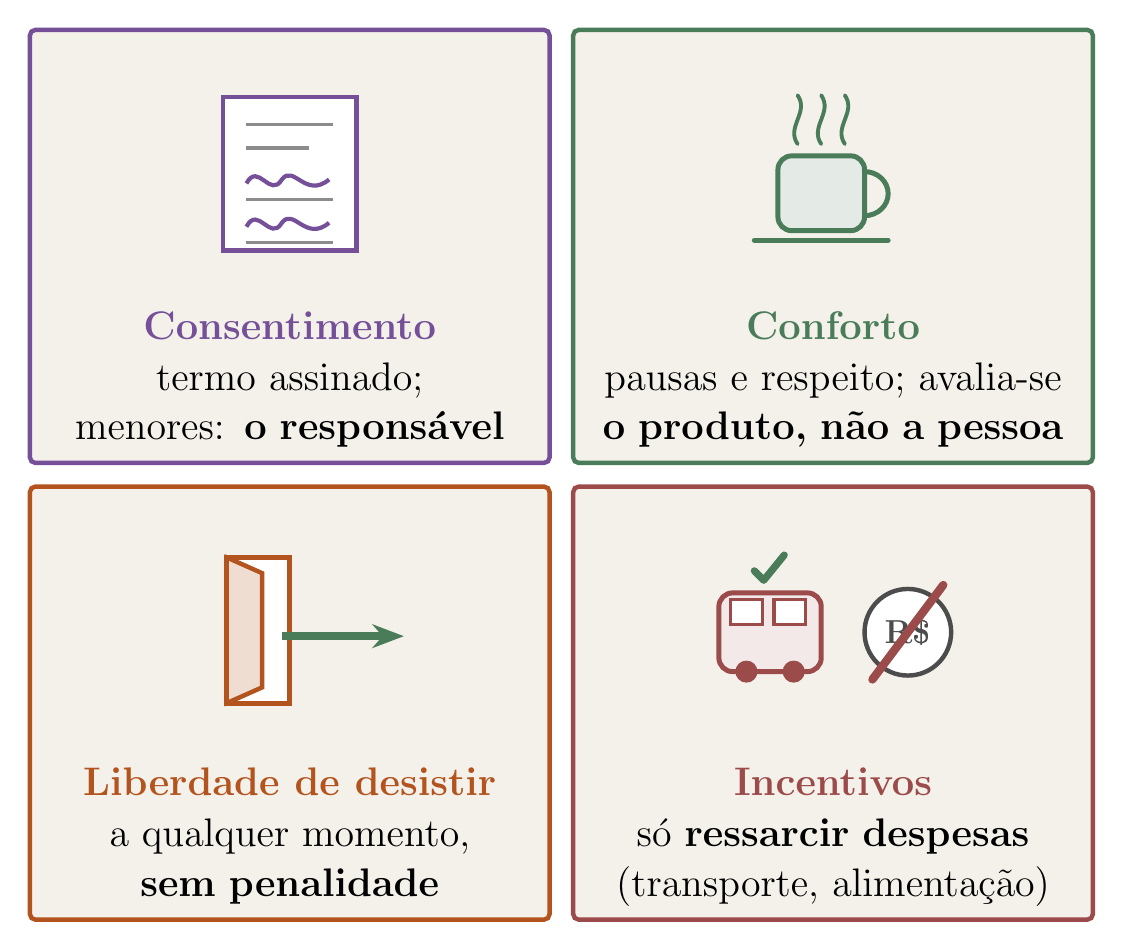
\begin{tikzpicture}[x=1cm,y=1cm]
\node[dbox, draw=dblue, line width=1.6pt, minimum width=6.6cm, minimum height=5.5cm] at (3.30,8.55) {};
\node[font=\Large\bfseries, dblue] at (3.30,7.55) {Consentimento};
\node[font=\Large, text width=6.0cm, align=center, anchor=north] at (3.30,7.20) {termo assinado; menores: \textbf{o responsável}};
\draw[dblue, fill=white, line width=1.6pt] (2.45,8.50) rectangle (4.15,10.45);
\draw[black!45, line width=1.2pt] (2.75,10.10) -- ++(1.10,0);
\draw[black!45, line width=1.2pt] (2.75,9.80) -- ++(0.80,0);
\draw[dblue, line width=1.5pt] (2.75,9.35) .. controls (2.90,9.63) and (3.05,9.15) .. (3.20,9.40) .. controls (3.35,9.60) and (3.50,9.15) .. (3.80,9.40);
\draw[black!45, line width=1pt] (2.75,9.15) -- ++(1.1,0);
\draw[dblue, line width=1.5pt] (2.75,8.80) .. controls (2.90,9.08) and (3.05,8.60) .. (3.20,8.85) .. controls (3.35,9.05) and (3.50,8.60) .. (3.80,8.85);
\draw[black!45, line width=1pt] (2.75,8.60) -- ++(1.1,0);
\node[dbox, draw=dgreen, line width=1.6pt, minimum width=6.6cm, minimum height=5.5cm] at (10.20,8.55) {};
\node[font=\Large\bfseries, dgreen] at (10.20,7.55) {Conforto};
\node[font=\Large, text width=6.0cm, align=center, anchor=north] at (10.20,7.20) {pausas e respeito; avalia-se \textbf{o produto, não a pessoa}};
\draw[dgreen, fill=dgreen!15!white, line width=1.8pt, rounded corners=5pt] (9.50,8.75) rectangle (10.60,9.70);
\draw[dgreen, line width=1.8pt] (10.60,9.50) arc (90:-90:0.3 and 0.28);
\draw[dgreen, line width=1.8pt, line cap=round] (9.20,8.63) -- (10.90,8.63);
\draw[dgreen, line width=1.4pt, line cap=round] (9.75,9.85) .. controls (9.60,10.07) and (9.90,10.25) .. (9.75,10.47);
\draw[dgreen, line width=1.4pt, line cap=round] (10.05,9.85) .. controls (9.90,10.07) and (10.20,10.25) .. (10.05,10.47);
\draw[dgreen, line width=1.4pt, line cap=round] (10.35,9.85) .. controls (10.20,10.07) and (10.50,10.25) .. (10.35,10.47);
\node[dbox, draw=dorange, line width=1.6pt, minimum width=6.6cm, minimum height=5.5cm] at (3.30,2.75) {};
\node[font=\Large\bfseries, dorange] at (3.30,1.75) {Liberdade de desistir};
\node[font=\Large, text width=6.0cm, align=center, anchor=north] at (3.30,1.40) {a qualquer momento, \textbf{sem penalidade}};
\draw[dorange, fill=white, line width=1.8pt] (2.50,2.75) rectangle (3.30,4.60);
\draw[dorange, fill=dorange!20!white, line width=1.6pt] (2.50,2.75) -- (2.95,2.95) -- (2.95,4.40) -- (2.50,4.60) -- cycle;
\draw[dgreen, line width=3pt, -{Stealth[length=4mm]}] (3.20,3.60) -- (4.75,3.60);
\node[dbox, draw=dred, line width=1.6pt, minimum width=6.6cm, minimum height=5.5cm] at (10.20,2.75) {};
\node[font=\Large\bfseries, dred] at (10.20,1.75) {Incentivos};
\node[font=\Large, text width=6.0cm, align=center, anchor=north] at (10.20,1.40) {só \textbf{ressarcir despesas} (transporte, alimentação)};
\draw[dred, fill=dred!12!white, line width=1.8pt, rounded corners=5pt] (8.75,3.15) rectangle (10.05,4.15);
\draw[dred, fill=white, line width=1.2pt] (8.90,3.75) rectangle ++(0.4,0.32);
\draw[dred, fill=white, line width=1.2pt] (9.45,3.75) rectangle ++(0.4,0.32);
\fill[dred] (9.10,3.15) circle (0.14) (9.70,3.15) circle (0.14);
\draw[dgreen, line width=2.6pt, line cap=round, line join=round] (9.20,4.43) -- (9.32,4.31) -- (9.58,4.63);
\draw[black!70, fill=white, line width=1.6pt] (11.15,3.65) circle (0.55);
\node[font=\large\bfseries, black!70] at (11.15,3.65) {R\$};
\draw[dred, line width=3pt, line cap=round] (10.70,3.05) -- (11.60,4.25);
\end{tikzpicture}
\end{document}
